\documentclass[mat1]{fmfdelo}
% \documentclass[fin1]{fmfdelo}
% \documentclass[isrm1]{fmfdelo}
% \documentclass[mat2]{fmfdelo}
% \documentclass[fin2]{fmfdelo}
% \documentclass[isrm2]{fmfdelo}

% aktivirajte pakete, ki jih potrebujete
% \usepackage{tikz}
\usepackage{graphicx}

% za številske množice uporabite naslednje simbole
\newcommand{\R}{\mathbb R}
\newcommand{\N}{\mathbb N}
\newcommand{\Z}{\mathbb Z}
\newcommand{\C}{\mathbb C}
\newcommand{\Q}{\mathbb Q}

% matematične operatorje deklarirajte kot take, da jih bo Latex pravilno stavil
% \DeclareMathOperator{\conv}{conv}

% na razpolago so naslednja matematična okolja, ki jih kličemo s parom 
% \begin{imeokolja}[morebitni komentar v oklepaju] ... \end{imeokolja}
%
% definicija, opomba, primer, zgled, lema, trditev, izrek, posledica, dokaz
% 


% vstavite svoje definicije ...
%  \newcommand{}{}


% naslednje ukaze ustrezno napolnite
\avtor{Živa Urbančič} 

\naslov{Grupa kit in njene upodobitve}
\title{Braid group and her representations}

% navedite ime mentorja s polnim nazivom: doc.~dr.~Ime Priimek, 
% izr.~prof.~dr.~Ime Priimek, prof.~dr.~Ime Priimek
% uporabite le tisti ukaz/ukaze, ki je/so za vas ustrezni 
\mentor{izr. prof. dr. Sašo Strle}
% \mentorica{}
% \somentor{}
% \somentorica{}
% \mentorja{}{}
% \mentorici{}{}

\letnica{2016} % leto diplome

%  V povzetku na kratko opišite vsebinske rezultate dela. Sem ne sodi razlaga organizacije dela --
%  v katerem poglavju/razdelku je kaj, pač pa le opis vsebine.
\povzetek{}

%  Prevod slovenskega povzetka v angleščino. 
\abstract{}

% navedite vsaj eno klasifikacijsko oznako --
% dostopne so na www.ams.org/mathscinet/msc/msc2010.html
\klasifikacija{}
\kljucnebesede{} % navedite nekaj ključnih pojmov, ki nastopajo v delu
\keywords{} % angleški prevod ključnih besed


\begin{document}

\section{Uvod}

Teorija kit je močno povezana s teorijo vozlov, a je zanimiva in pomembna tudi kot samostojna raziskovalna smer. Kite je prvi definiral avstrijski matematik Emil Artin v svojem članku \emph{``Theorie der Z\''{o}pfe''}, ki je bil objavljen leta $1925$. Glavni izrek članka reši problem klasifikacije kit, a z njegovim dokazom Artin ni bil zadovoljen. Opisal ga je kot ``neprepričljivega'' in ga nato v članku z naslovom \emph{``Theory of braids''}(1947) zapisal na način, ki prepriča tudi najbolj rigorozne in skeptične bralce. Tako je teorijo pravzaprav postavil na njene temelje. Leta raziskovanja so prinesla tudi nekatere ekvivalentne definicije, ki so jih matematiki prilagodili potrebam preučevanja in uporabe v drugih matematičnih in z matematiko povezanih smereh. Uporablja se recimo v mehaniki fluidov, statistični mehaniki, nekomutativni kriptografiji, \ldots

%\section{Prosta grupa in upodobitve}
%
%To poglavje je namenjeno razlagi algebraične teorije, ki jo bomo potrebovali za nadaljne raziskovanje. Vpeljali bomo pojme, ki jih potrebujemo, da lahko definiramo, kaj je upodobitev in jo kasneje tudi poiščemo.\\
%Naj bo $X = \{ x_1,\ x_2,\ \ldots,\ x_n \}$ neka množica (lahko je tudi neskončna). Imenujmo jo \emph{abeceda}, posamezen element pa imenujmo \emph{črka}. Definirajmo množico $S$ kot množico vseh besed, ki jih lahko sestavimo iz črk abecede $X$.
%
%\begin{trditev}
%Množica $S$ je za operacijo stikanja besed ($x \circ y = xy, \ x, y \in X$) polgrupa.
%\end{trditev}
%
%\begin{dokaz}
%Operacija je očitno asociativna.
%\end{dokaz}
%
%\begin{opomba}
%Polgrupo $(S, \circ)$ imenujemo \emph{prosta polgrupa}.
%\end{opomba}
%
%\begin{opomba}
%Če množici $S$ dodamo še prazno besedo, postane za operacijo stikanja monoid.
%\end{opomba}
%
%Vprašanje, kaj $S$ (z dodano prazno besedo) manjka do grupe, nas motivira k definiciji množice $X^{-1} = \{x_1^{-1},\ x_2^{-1}, \ \ldots, \ x_n^{-1}\}$. Nova abeceda naj bo $A = X \cup X^{-1}$. Množica besed nad $A$ pa še ni, kar iščemo, saj v besedah ne želimo podbesed oblike $x_ix_i^{-1}$.
%
%\begin{definicija}
%Beseda nad $A$ je \emph{reducirana}, če ne vsebuje podbesede oblike $xx^{-1}$ ali $x^{-1}x$, kjer je $x\in A$.
%\end{definicija}
%
%Označimo z $F_x$ množico vseh reduciranih besed nad $A$. Na njej definirajmo operacijo $\circ$, ki stakne besedi in ju zapiše v reducirani obliki (tj. pokrajša neželene podbesede).
\break
\section{Grupa kit}

\subsection{Definicija grupe kit}

Kot je bilo omenjeno v uvodu, lahko grupo kit definiramo na različne (ekvivalentne) načine, kakor najbolj ustreza našemu raziskovanju. V tem razdelku bomo podali geometrijsko definicijo kite (nekatere druge bralec lahko najde v \cite{Manturov}) in se prepričali, da množica kit, če na njej definiramo operacijo stikanja, res postane grupa. Pri tem bomo morali obravnavati tudi, kdaj sta kiti ekvivalentni, pri čemer bomo sledili \cite{Burde} in \cite{Manturov}.\\
Kite si lahko zelo naravno predstavljamo kot skupek pramenov, ki so prepleteni med seboj. To je zgolj opis, za podrobnejše preučevanje potrebujemo bolj formalno in matematično korektno definicijo.\\
Na vsaki izmed premic $\{y = z = 0\}$ ter $\{y = 0, z = 1\}$, ki sta vloženi v $\R^3$, izberemo $m$ točk z abscisami $x=1,\ 2,\ \ldots,\ m$.

\begin{definicija}
\emph{Kita z m prameni} je množica $m$ disjunktnih gladkih poti - imenujemo jih \emph{prameni}, ki povezujejo točke s prve izbrane premice s tistimi z druge (v poljubnem vrstnem redu). Projekcija posameznega pramena na os $z$ mora biti difeomorfizem.
\end{definicija}

\begin{figure}[ht!]
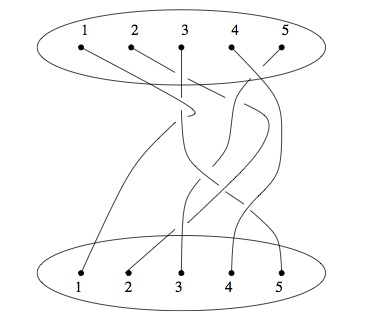
\includegraphics[height = 5cm]{Primer_kite_1}
\caption{Primer kite s 5 prameni.}
\end{figure}

\begin{opomba}
Zahteva, da je projekcija vsakega od pramenov na $z$ os difeomorfizem, v resnici pomeni, da prameni monotono padajo (če izberemo parametrizacijo kot v definiciji, tj. od točk na $\{y = 0, z = 1\}$ do tistih na $\{y = z = 0\}$). Enostavneje, nobeden izmed pramenov ne zavije navzgor, kot je prikazano na spodnji sliki.
\end{opomba}

\begin{figure}[h!]
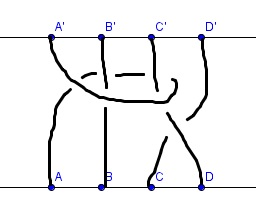
\includegraphics[height = 4.3cm]{ne-kita}
\caption{Projekcija pramena, ki se začne v $A'$ in konča v $A$, na os $z$ ni difeomorfizem.}
\end{figure}

\begin{primer}
Oglejmo si enostaven primer kit $B_0$ in $B_1$ s spodnje slike. Zelo enostavno je videti, da prvo kito lahko ``odpletemo'' v drugo, ne da bi kakšen pramen pretrgali ali da bi spreminjali njegovo začetno ali končno točko. Sklepamo, da sta na nek način sorodni.
\end{primer}

\begin{figure}[h!]
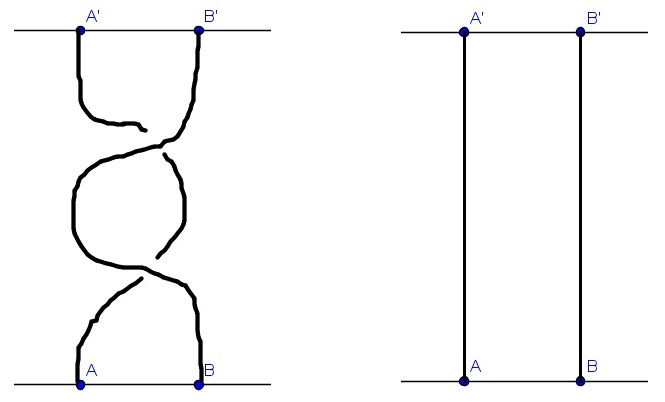
\includegraphics[height = 4cm]{Primer_3}
\caption{Kiti $B_0$ in $B_1$.}
\end{figure}

Naravno vprašanje, ki sledi zgornjemu primeru je, katere kite so si sorodne oziroma kako lahko deformiramo kito, da se ohranijo njene lastnosti? Da lahko na to vprašanje odgovorimo, vpeljimo nekaj topoloških pojmov.

\begin{definicija}
Vložitvi $f_0,f_1: X \rightarrow Y$ sta \emph{izotopni}, če obstaja taka vložitev $F: X \times I \rightarrow Y\times I$, da je
$$F(x, t)=(f(x,t), t),$$ kjer je $x \in X$, $t \in I$, $f(x,0)=f_0(x)$ in $f(x,1)=f_1(x)$. Tako vložitev F imenujemo \emph{level-preserving izotopija}.
\end{definicija}

\begin{opomba}
Definicija bolj enostavno povedano pomeni, da vložitvi $f_0$ in $f_1$ lahko povežemo z vložitvami.
\end{opomba}

\begin{opomba}
Zaradi enostavnosti zapisa namesto $f(x,t)$ pišemo $f_t(x)$.
\end{opomba}

Izotopija zvezno ``premika'' $f_0$ k $f_1$, a ne pazi na to, kaj se dogaja v ciljnem prostoru v bližini slike vložitve. Zakaj to predstavlja problem, si oglejmo na naslednjem primeru.

\begin{figure}[h!]
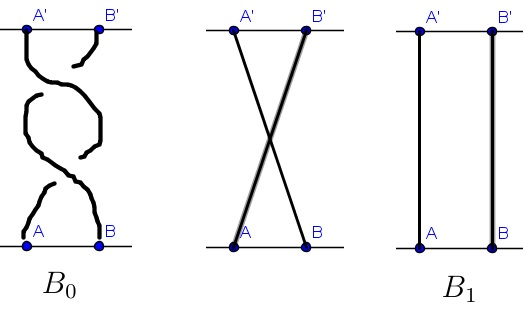
\includegraphics[height = 4cm]{Primer_2}
\caption{Kita $B_0$, vmesni korak in kita $B_1$.}
\end{figure}

\begin{primer}
Oglejmo si kiti $B_0$ in $B_1$ z zgornje slike. Jasno je, da moramo, če želimo eno zvezno preoblikovati v drugo, prekiniti pramen ali ga ``odlepiti'' od ene od fiksnih premic z začetnimi in končnimi točkami. A med njima obstaja izotopija, ki pramena tako približa, da se obe menjavi kite $B_0$ vršita v isti točki, kar prikazuje vmesni korak na zgornji sliki.
\end{primer}

Očitno je, da izotopnosti ne moremo vzeti za definicijo ekvivalence kit. Če želimo, da se bodo ohranjali prepleti, ki jih ne moremo razplesti, brez da bi pretrgali pramene, mora namreč preslikava nositi tudi nekaj informacij o ciljnem prostoru.

\begin{definicija}
Vložitvi $f_0,f_1: X \rightarrow Y$ sta \emph{ambientno izotopni}, če obstaja level-preserving izotopija $H: Y \times I \rightarrow Y\times I$, da je
$$H(y,t)=(h_t(y),t),$$ kjer je $f_1=h_1 \circ f_0$ in $h_0=id_y$. Preslikavo $H$ imenujemo \emph{ambientna izotopija}.
\end{definicija}

\begin{opomba}
Namesto, da bi preoblikovali vložitev, sedaj preoblikujemo cel prostor. Preoblikovanje vložitve je posledica preoblikovanja ciljnega prostora.
\end{opomba}
%S tem smo definirali izotopijo $F$, ki povezuje $f_0$ in $f_1$, kot $F(x,t)=H(h_t \circ f_0(x), t)$.


\begin{definicija}
Kiti $B_0$ in $B_1$ sta \emph{ekvivalentni}, če sta \emph{izotopni}.
\end{definicija}

\begin{opomba}
Enostavneje zgornja definicija pove, da eno vložitev kite lahko zvezno deformiramo v drugo.
\end{opomba}

%\begin{opomba}
%Od sedaj naprej, bomo izraz izraz\˝ kita \˝ uporabljali za ekvivalenčni razred kit.
%\end{opomba}
%--------------------------------------------------------------------------------

Naj bosta $B_0$ in $B_1$ kiti z $n$ prameni. Z $\gamma_i$ označimo pramen $B_0$, ki se začne v $(i, 0, 1)$, konča pa se v $(j, 0, 0)$, kjer je $j$ poljuben element $\{1, \ldots, n\}$. S $\theta_i$ označimo pramen $B_1$, ki se začne v $(j, 0, 1)$. Iz $B_0$ in $B_1$ lahko dobimo novo kito tako, da staknemo $\gamma_i$ in $\theta_i$ za vsak $i=1, \ldots, n$.  Označimo jo z $B_0*B_1$.

\begin{figure}[ht!]
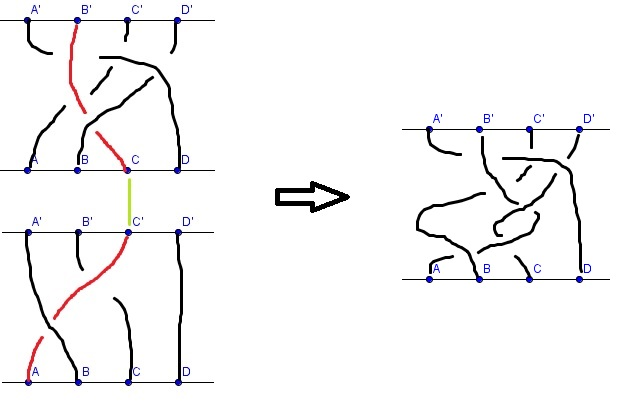
\includegraphics[height = 7cm]{Stikanje_2}
\caption{Stik pramenov $\gamma_2$ in $\theta_2$ in kita, ki jo dobimo s stikom vseh pramenov $B_0$ in $B_1$.}
\end{figure}

%Operacija stikanja je DD.

\begin{trditev}
Množica ekvivalenčnih razredov kit z $n$ prameni je za operacijo stikanja grupa.
\end{trditev}

\begin{dokaz}
Najprej moramo preveriti, da je operacija sploh dobro definirana, nato pa še, da množica ekvivalenčnih razredov z operacijo stikanja zadosti kriterijem za grupo.
\begin{itemize}
\item{Oglejmo si kite $A_0$, $A_1$, $B_0$ in $B_1$, za katere velja: $$A_0 \cong A_1 \ \text{in} \ B_0 \cong B_1.$$ Pokazati želimo, da sta kiti $A_0*B_0$ in $A_1*A_2$ ekvivalentni. }
\item{Stikanje je očitno asociativna operacija.}
\item{Enota}
\item{Inverz}
\end{itemize}
\end{dokaz}

\begin{figure}[ht!]
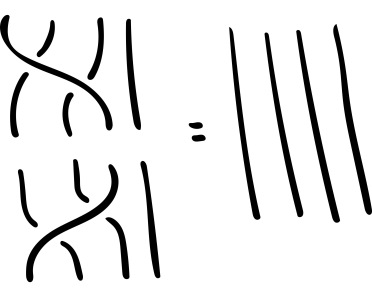
\includegraphics[height=4cm]{Inverz_1}
\caption{Inverzni element in enota.}
\end{figure}


\subsection{Lastnosti grupe kit}


\section{Upodobitve grupe kit}

\subsection{Artinove relacije}

Delo z ekvivalenčnimi razredi je lahko zamudno in težavno, zato si kite poskušamo predstavljati drugače. O kitah lahko razmišljamo kot o zaporedju menjav. 

\begin{definicija}
\emph{Grupo kit z $m$ prameni} podamo z $(m - 1)$ generatorji $\sigma_1,\ \ldots ,\ \sigma_{m - 1}$, za katere veljata relaciji: $$ \sigma_i \sigma_j = \sigma_j \sigma_i $$ za vsaka $i$ in $j$, za katera je $|i - j| \geq 2$ in $$\sigma_i \sigma_{i+1} \sigma_i = \sigma_{i+1} \sigma_i \sigma_{i+1}$$ za vsak $i = 1,\ 2,\ \ldots,\ m-2$.
\end{definicija}

\begin{opomba}
Zgornji relaciji imenujemo \emph{Artinovi relaciji}.
\end{opomba}

\subsection{Buraujeva upodobitev}

\subsection{Upodobitev Krammer\-Bigelow}





\section*{Slovar strokovnih izrazov}

%\geslo{Živa}{Najboljša v vsem ever.}
\geslo{Pramen}{}
\geslo{Difeomorfizem}{}
\geslo{Kita}{}
\geslo{(Gladka) pot}{}
\geslo{Grupa}{}
\geslo{Izotopnost}{}
\geslo{Ekvivalenčna relacija}{}
\geslo{Ekvivalenčni razred}{}
\geslo{Generatorji grupe}{}
\geslo{Artinove relacije}{}





% seznam uporabljene literature
\begin{thebibliography}{99}
\bibitem{Burde}{G. Burde, H. Zieschang. {\em Knots}, 2nd ed. Walter de Gruyter, Berlin, 2003.}
\bibitem{Manturov}{V. O. Manturov. {\em Knot Theory}, 1st ed. CRC Press, 2004. Dostopno na \url{http://varf.ru/rudn/manturov/book.pdf}.}
\bibitem{Wiki_braid_theory}{\emph{Braid theory}, v: Wkipedia: The Free Encyclopedia, [ogled 11. 11. 2016], dostopno na \url{https://en.wikipedia.org/wiki/Braid_theory}.}

\end{thebibliography}

\end{document}